% ----------------------------------------------------------
\section{Análise dos dados de Material Particulado}
% ----------------------------------------------------------

A Figura \ref{fig:data-pm10-raw} mostra a série temporal do sensor de \acrshort{mp10} depois de removidos os valores fora de intervalo. Os resultados do pré-processamento das leituras do sensor são ilustrados nas Figuras \ref{fig:data-pm10-preproc-hist} e \ref{fig:data-pm10-preproc-15} que apresentam, respectivamente, o histograma dos dados e a série pré-processada do sensor OPC-N3 juntamente com o comportamento diário das medições ao longo do período agrupadas por hora do dia.

O sensor de material particulado é um sensor digital com algoritmos próprios de filtragem, correção e ajuste de linha base. Por esse motivo, as leituras do sensor não apresentaram alterações na linha base nem foram tão ruidosas como as dos sensores eletroquímicos. Da mesma forma não é possível identificar um padrão de comportamento diário tão claro quanto os outros sensores. Em comparação com o comportamento diário das leituras de referência (Figura \ref{fig:data-pm10-reference}) observa-se que estas também não apresentaram um padrão diário muito evidente.

\begin{figure}[h!]
    \centering
    \caption{Série temporal das leituras do sensor OPC-N3}
    \begin{subfigure}{0.495\textwidth}
        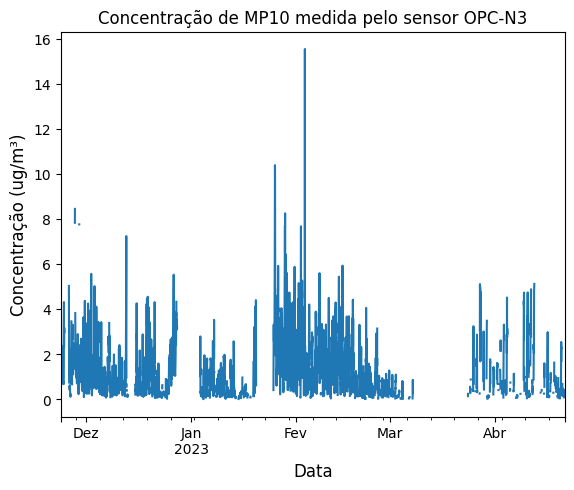
\includegraphics[width=\textwidth]{chapters/3-ANÁLISE DOS DADOS/Figuras/raw-pm10.png}
        \caption{Série temporal do sensor depois de remover valores fora de intervalo}
        \label{fig:data-pm10-raw}
    \end{subfigure}
    \hfill
    \begin{subfigure}{0.495\textwidth}
        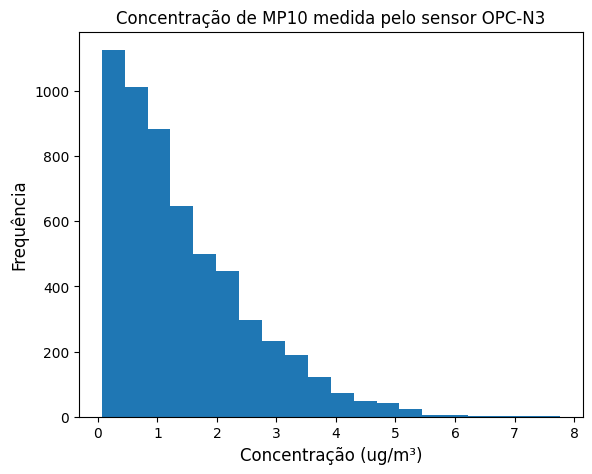
\includegraphics[width=\textwidth]{chapters/3-ANÁLISE DOS DADOS/Figuras/preproc-hist-pm10.png}
        \caption{Histograma das leituras pré-processadas do sensor OPC-N3}
        \label{fig:data-pm10-preproc-hist}
    \end{subfigure}
    \hfill
    \begin{subfigure}{0.99\textwidth}
        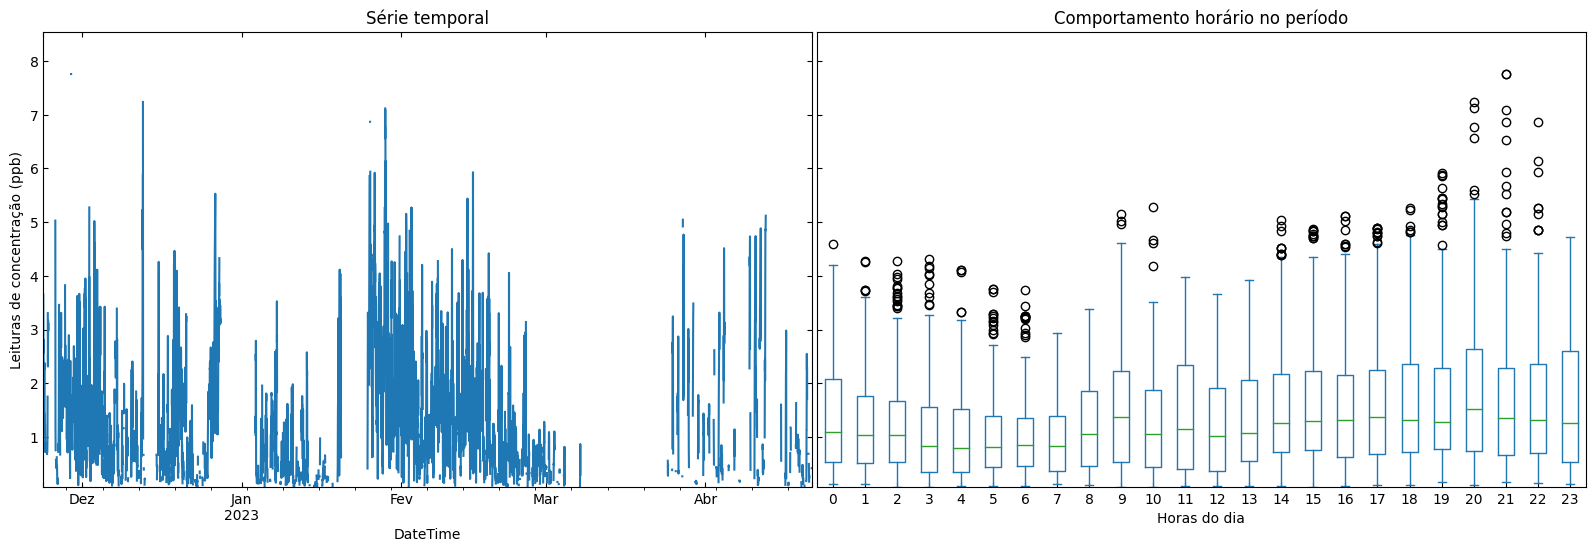
\includegraphics[width=\textwidth]{chapters/3-ANÁLISE DOS DADOS/Figuras/preproc-pm10.png}
        \caption{Série temporal do sensor pré-processada (T = 15 mins) e seu comportamento diário}
        \label{fig:data-pm10-preproc-15}
    \end{subfigure}
    \hfill
    \begin{subfigure}{0.99\textwidth}
        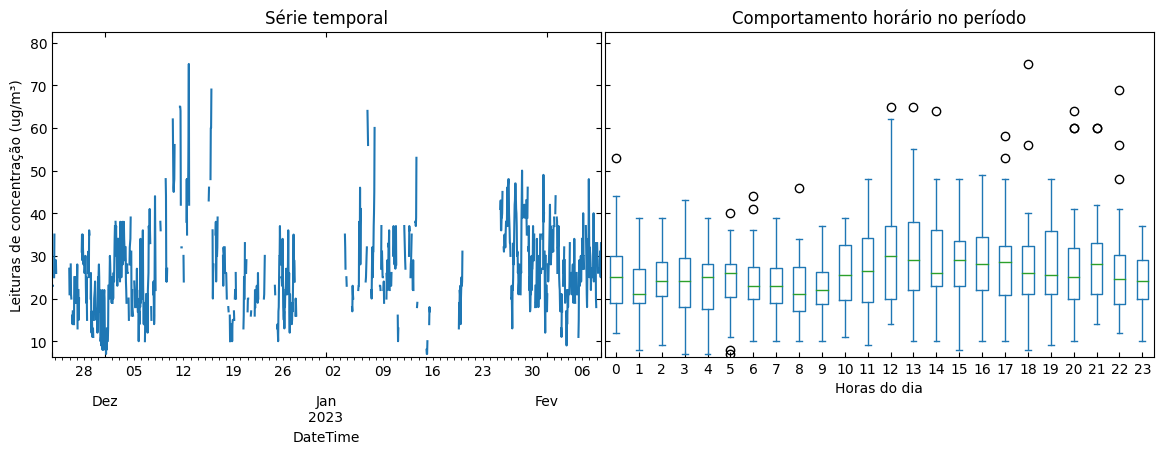
\includegraphics[width=\textwidth]{chapters/3-ANÁLISE DOS DADOS/Figuras/pm10-reference-series-and-box.png}
        \caption{Série temporal das leituras de concentração de referência (T = 1 H) e seu comportamento diário}
        \label{fig:data-pm10-reference}
    \end{subfigure}
    \hfill
    \label{fig:data-pm10}
\end{figure}

\begin{figure}[h!]
    \centering
    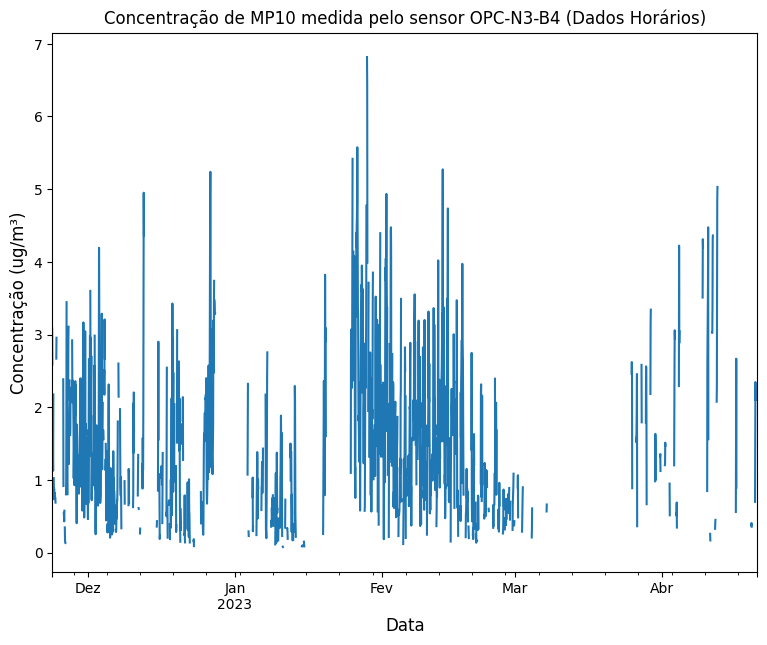
\includegraphics[width=0.5\textwidth]{chapters/3-ANÁLISE DOS DADOS/Figuras/preproc-1HR-pm10.png}
    \caption{Série temporal com T = 1 hr}
    \label{fig:data-pm10-preproc-1HR}
\end{figure}

Os dados do sensor de \acrshort{mp10} do OPC-N3 foram re-amostrados para um período de 1 hora para serem calibrados com as leituras de referência; a Figura \ref{fig:data-pm10-preproc-1HR} mostra a série temporal resultante da re-amostragem.

Na Tabela \ref{tab:data-contab-pm10} contabilizam-se os dados para períodos de 15 minutos e de 1 hora. Observa-se que dos 14541 pontos de dados, que representavam as amostras adquiridas com um período de 15 minutos no intervalo de 21/11/2022 até 21/04/2023, 5668 foram aproveitados como dados válidos, o que representa um 39 \% aproximadamente dos dados originais. Ao re-amostrar esses 5668 pontos em dados horários obtiveram-se 1291 amostras horárias de concentração válidas (aproximadamente 36 \% dos dados) para realizar a calibração. Vale salientar que nos dados de \acrshort{mp10} não foram encontradas alterações na linha base nem dados de estabilização já que esse sensor não precisa desse intervalo prévio as medições.

\begin{table}[h!]
    \caption{Contabilização dos dados por etiquetas das leituras de \acrshort{mp10} do sensor OPC-N3}
    \centering
    \begin{tabularx}{0.95\textwidth}[h]{
         >{\raggedright\hsize=.475\hsize\arraybackslash}X
         >{\raggedright\hsize=.20\hsize\arraybackslash}X 
         >{\raggedright\hsize=.5\hsize\arraybackslash}X
        | >{\raggedright\hsize=.50\hsize\arraybackslash}X 
         >{\raggedright\hsize=.20\hsize\arraybackslash}X 
         >{\raggedright\hsize=.5\hsize\arraybackslash}X }
        \multicolumn{3}{c|}{Série temporal T = 15 mins} & \multicolumn{3}{c}{Série temporal T = 1 hr} \\
        \hline
        Etiquetas & No. amostras & \% amostras & Etiquetas & No. amostras & \% amostras \\ [0.5ex]
        \hline
        \textit{MISSING} & 6481 & 44.57 \% & \textit{LOWSAMPLES} & 2291 & 63.96 \% \\ [0.5ex]
        
        \textit{LTLL} & 1759 & 12.10 \% & \textit{VALID} & 1291 & 36.04 \% \\ [0.5ex]
        
        \textit{GTUL} & 0 & 0.0 \% & & & \\ [0.5ex]
        
        \textit{STABILIZING} & 0 & 0.0 \% & & & \\ [0.5ex]
        
        \textit{BADSPIKE} & 430 & 2.96 \% & & & \\ [0.5ex]
        
        \textit{LTQTLE01} & 117 & 0.80 \% & & & \\ [0.5ex]
        
        \textit{GTQTLE99} & 86 & 0.59 \% & & & \\ [0.5ex]
        
        \textit{REBASE} & 0 & 0.0 \% & & & \\ [0.5ex]
        
        \textit{VALID} & 5668 & 38.98 \% & & & \\ [0.5ex]
        \hline
        TOTAL & 14541 & & TOTAL & 3582 & \\
    \end{tabularx}
    \label{tab:data-contab-pm10}
\end{table}

\subsubsection{Dependência com a temperatura}

Investigou-se a existência de correlação entre as leituras do sensor de \textit{mp10} e as variações de temperatura medida no interior da câmara de medição. Os resultados dos testes estatísticos de Spearman e Kendall revelaram coeficientes de correlação estatisticamente significativos, conforme se ilustra na Figura \ref{fig:data-temp-pm10-corr}. O coeficiente de Spearman resultou em 0.29 com um valor de p inferior a 0.05, indicando uma correlação estatisticamente significativa entre as leituras dos sensores e a temperatura. De maneira semelhante, o coeficiente de Kendall foi de 0.20, também com p < 0.05, reforçando a presença de uma associação significativa. Ao avaliar a hipótese nula de ausência de correlação, os resultados forneceram evidências para sua rejeição, sugerindo a existência de uma correlação entre as leituras dos sensores de \acrshort{mp10} e as variações de temperatura.

\begin{figure}[h]
    \centering
    \caption{Relação dos dados de concentração de \acrshort{mp10} com a temperatura}
    \begin{subfigure}{0.4\textwidth}
        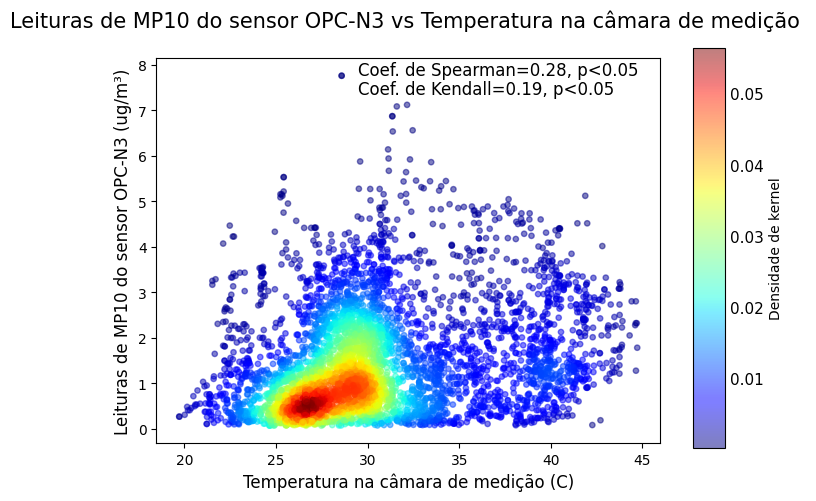
\includegraphics[width=\textwidth]{chapters/3-ANÁLISE DOS DADOS/Figuras/temperature-pm10.png}
        \caption{Relação entre as leituras do sensor OPC-N3 e a temperatura}
        \label{fig:data-temp-pm10-corr}
    \end{subfigure}
    \hfill
    \begin{subfigure}{0.4\textwidth}
        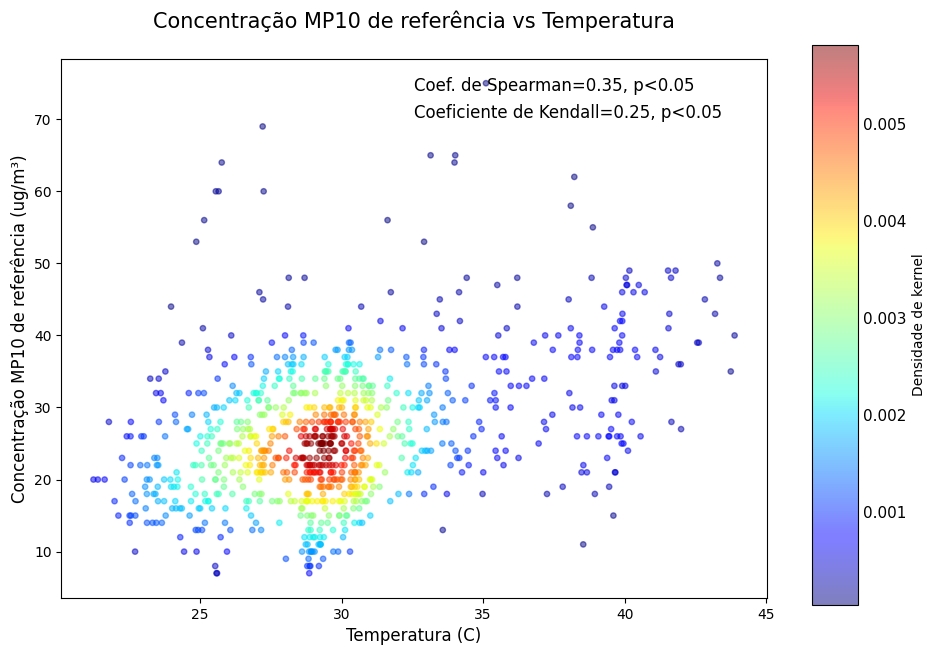
\includegraphics[width=\textwidth]{chapters/3-ANÁLISE DOS DADOS/Figuras/temperature-pm10-reference.png}
        \caption{Relação entre os valores de concentração de referência e a temperatura}
        \label{fig:data-temp-pm10-ref-corr}
    \end{subfigure}
    \hfill
    \label{fig:data-pm10-temp}
\end{figure}

Os resultados obtidos nos testes estatísticos podem ser corroborados no gráfico de dispersão entre as variáveis. Na Figura \ref{fig:data-temp-pm10-corr} observa-se que o núcleo principal dos dados de concentração, entre 0 e 2 \(\mu g/m^3\), mostrou uma tendência crescente com as variações de temperatura entre 25 a 30\textdegree C. Da mesma forma, ao analisar a relação entre as medições de concentração de referência e a temperatura, observa-se correlação, com coeficientes de Spearman e Kendall de 0.35 e 0.25 respectivamente (Figura \ref{fig:data-temp-pm10-ref-corr}).

\subsection{Calibração das leituras de \acrshort{mp10} do sensor OPC-N3 com as medições de referência}

Nas Figuras \ref{fig:data-pm10-reference-time-series} e \ref{fig:data-pm10-reference-corr} apresentam-se as leituras de \acrshort{mp10} obtidas pelo sensor OPC-N3 de Alphasense e a estação de referência. Observa-se que as leituras do sensor OPC-N3 subestimaram os valores de concentração de referência com valores aproximadamente 10 vezes menores. Os testes de Spearman e Kendall revelaram a existência de correlação entre as medições com o sensor de baixo custo e a referência com coeficientes de 0.3 e 0.2 respectivamente.

\begin{figure}[h!]
    \centering
    \caption{Séries temporais e gráficos de dispersão das medições de \acrshort{mp10}}
    \begin{subfigure}{0.44\textwidth}
        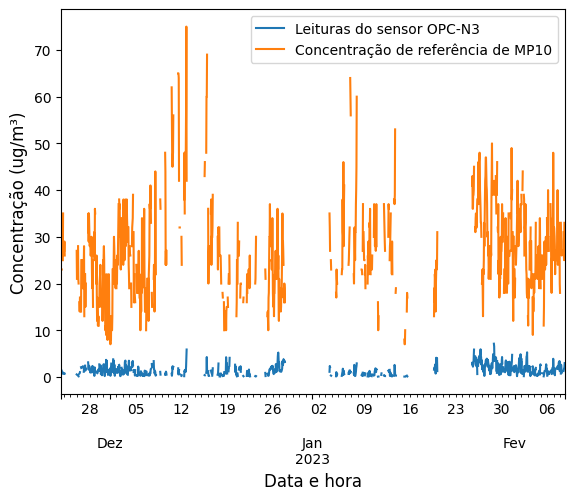
\includegraphics[width=\textwidth]{chapters/3-ANÁLISE DOS DADOS/Figuras/pm10-reference-time-series.png}
        \caption{Séries temporais das leituras de \acrshort{mp10} do sensor OPC-N3 e a estação de referência}
        \label{fig:data-pm10-reference-time-series}
    \end{subfigure}
    \hfill
    \begin{subfigure}{0.54\textwidth}
        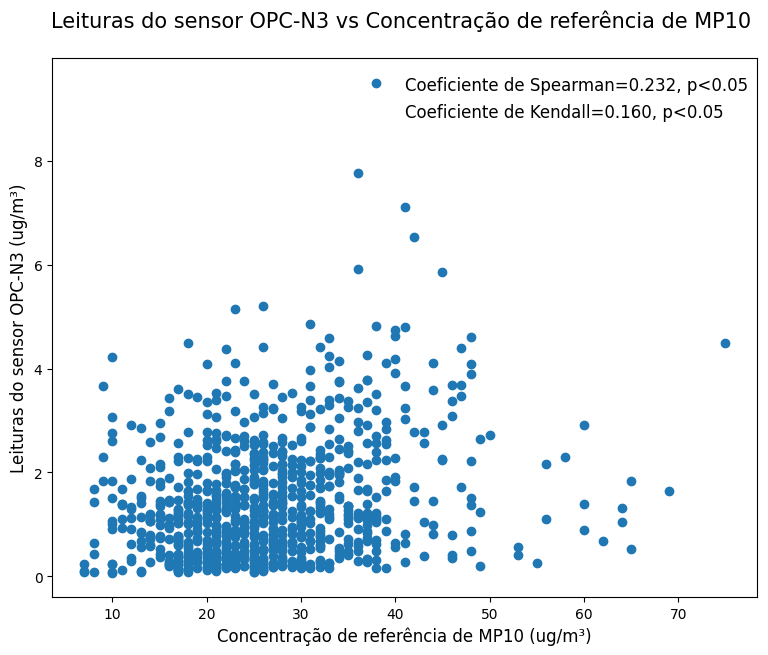
\includegraphics[width=\textwidth]{chapters/3-ANÁLISE DOS DADOS/Figuras/pm10-reference-correlation.png}
        \caption{Gráfico de dispersão das leituras de \acrshort{mp10} do sensor OPC-N3 e a estação de referência}
        \label{fig:data-pm10-reference-corr}
    \end{subfigure}
\end{figure}

\begin{table}[h!]
    \caption{Resultados da calibração das leituras de \acrshort{mp10} do sensor OPC-N3}
    \centering
    \begin{tabularx}{0.95\textwidth}[h!]{
        >{\raggedright\hsize=.4\hsize\arraybackslash}X
        >{\raggedright\hsize=.6\hsize\arraybackslash}X 
        >{\raggedright\hsize=.6\hsize\arraybackslash}X
        >{\raggedright\hsize=.7\hsize\arraybackslash}X 
        >{\raggedright\hsize=.6\hsize\arraybackslash}X 
        >{\raggedright\hsize=.3\hsize\arraybackslash}X }
        \hline
        Var. & Modelo & R2 & RMSE & MAE & $\rho$\\ [0.5ex]
        \hline
        \acrshort{mp10} & \textbf{MLP}: & -0.05 ± 0.036 & -9.77 ± 0.75 & -7.41 ± 0.49 & 0.18 \\ [0.5ex]
           & \textbf{MLR} & -0.01 ± 0.03 & -9.57 ± 0.98 & -7.26 ± 0.62 & 0.17 \\ [0.5ex]
           & \textbf{KNN:} & -0.14 ± 0.07 & -10.18 ± 0.62 & -7.71 ± 0.45 & 0.13 \\ [0.5ex]
           & \textbf{RF:} & -0.19 ± 0.11 & -10.33 ± 0.52 & -7.80 ± 0.40 & 0.22\\ [0.5ex]
        \hline
        \acrshort{mp10}, T & \textbf{MLP:} & -0.29 ± 0.27 & -10.68 ± 0.96 & -8.33 ± 0.78 & 0.47 \\ [0.5ex]
              & \textbf{MLR:} & 0.10 ± 0.08 & -9.04 ± 1.12 & -6.73 ± 0.69 & 0.37 \\ [0.5ex]
              & \textbf{KNN:} & -0.02 ± 0.09 & -9.57 ± 0.46 & -7.29 ± 0.27 & 0.45 \\ [0.5ex]
              & \textbf{RF:} & -0.17 ± 0.27 & -10.12 ± 0.32 & -7.89 ± 0.28 & 0.46 \\ [0.5ex]
        \hline
    \end{tabularx}
    \label{tab:data-pm10-calib-results}
\end{table}

A partir dos dados de referência e das leituras de concentração e temperatura adquiridas pelo monitor em questão, foi realizada uma busca em grid para encontrar as melhores combinações de parâmetros e variáveis de entrada a modelos de regressão. As variáveis que foram testadas como entrada foram as leituras de concentração de \acrshort{mp10} do sensor OPC-N3 e a temperatura no interior da câmara de medição. Como modelos de regressão foram testados: o Perceptron Multicamadas (MLP), a Regressão Linear Multivariada (MLR), os K Vizinhos mais Próximos (KNN) e as Florestas Aleatórias (RF). Na Tabela \ref{tab:data-pm10-calib-results} resumem-se os melhores modelos encontrados pela busca em \textit{grid} para calibrar as leituras do sensor OPC-N3. Os mesmos resultados são ilustrados graficamente na Figura \ref{fig:data-pm10-models-performance} que apresenta o desempenho dos modelos e as variáveis de entrada considerando os valores de r2, RMSE e MAE.

\begin{figure}[h!]
    \centering
    \caption{Resultados dos modelos de calibração aplicados as leituras de \acrshort{mp10} do sensor OPC-N3}
    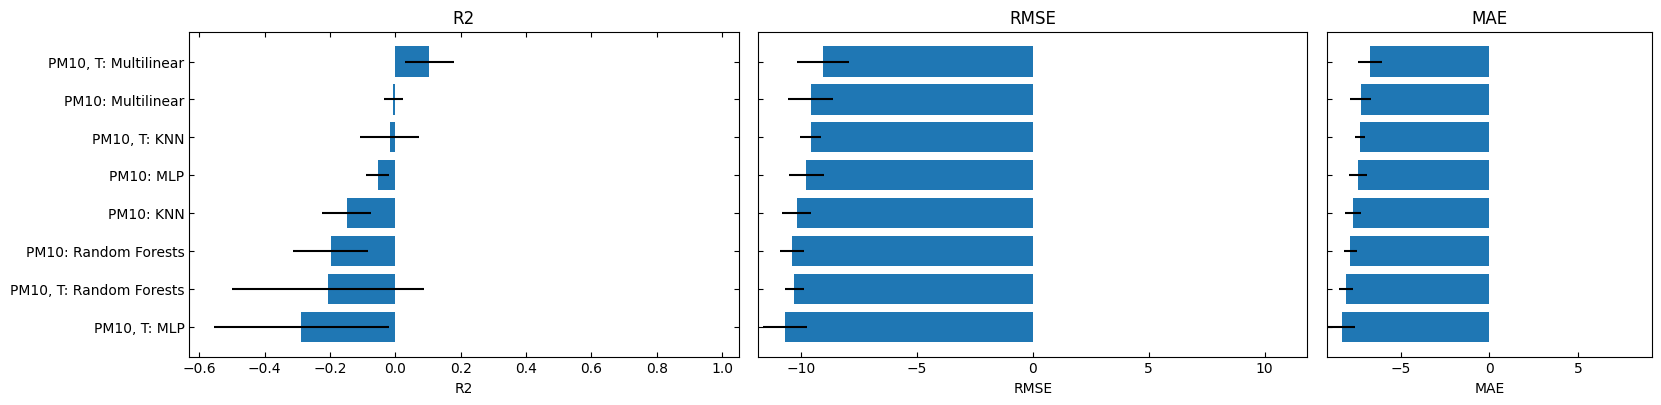
\includegraphics[width=0.95\textwidth]{chapters/3-ANÁLISE DOS DADOS/Figuras/pm10-models-performance.png}
    \label{fig:data-pm10-models-performance}
\end{figure}

\begin{figure}[h!]
    \centering
    \caption{Gráfico de dispersão das leituras do sensor de \acrshort{mp10} do OPC-N3 e a estação de referência após aplicar modelos de regressão considerando a temperatura}
    \begin{subfigure}{0.49\textwidth}
        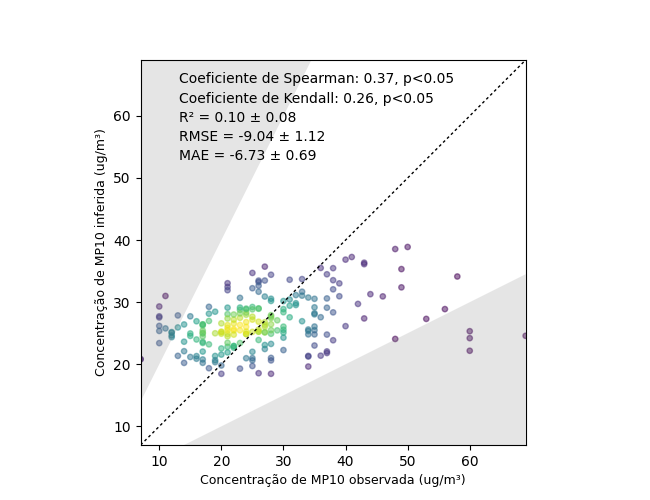
\includegraphics[width=\textwidth]{chapters/3-ANÁLISE DOS DADOS/Figuras/pm10-T-ML-Regression.png}
        \caption{Utilizando uma regressão linear multivariada considerando a temperatura obteve-se um R2 de 0.10 e $\rho$ de 0.37}
        \label{fig:data-pm10-T-reference-corr-MLR}
    \end{subfigure}
    \hfill
    \begin{subfigure}{0.49\textwidth}
        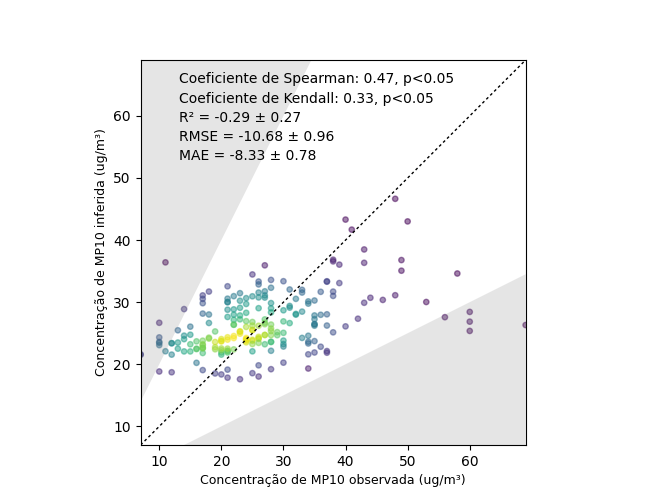
\includegraphics[width=\textwidth]{chapters/3-ANÁLISE DOS DADOS/Figuras/pm10-T-MLP-Regression.png}
        \caption{Utilizando uma rede neural Perceptron Multicamadas considerando a temperatura obtiveram-se valores de $\rho$ de 0.47 e 0.33}
        \label{fig:data-pm10-T-reference-corr-MLP}
    \end{subfigure}
\end{figure}
Como se observa, apenas o modelo de regressão linear com variáveis independentes temperatura e concentração medida pelo sensor OPC-N3 conseguiu explicar a variância na variável dependente, i.e. a concentração real. Os valores de R2 obtidos nas validações cruzadas realizadas para este modelo foram de 0.10 ± 0.08, e os coeficientes de correlação de Spearman e Kendall entre a concentração inferida na calibração e a concentração real foram de 0.37 e 0.26 respectivamente. Os erros RMSE e MAE estiveram próximos de 10 \(\mu g/m^3\), que é um valor relativamente baixo considerando a diferença elevada entre os valores de referência e as leituras do sensor (aproximadamente 10 vezes). De modo geral, os modelos não lineares que incluíram a temperatura como variável dependente, apresentaram melhorias na correlação entre a concentração real e a medida pelo sensor, com coeficientes de correlação de até 0.47. As Figuras \ref{fig:data-pm10-T-reference-corr-MLR} e \ref{fig:data-pm10-T-reference-corr-MLP} apresentam os resultados ao aplicar o modelo de regressão linear considerando leituras do sensor e temperatura e ao aplicar uma rede neural Perceptron Multicamadas considerando as mesmas variáveis de entrada.